\documentclass[a4paper,11pt]{article}
\usepackage{graphicx}
\usepackage{pifont}
\usepackage{ulem}
\voffset -1.5cm
\hoffset 0.0cm
\textheight 25cm
\textwidth 16cm
\topmargin 0.0cm
\oddsidemargin 0.0cm
\evensidemargin 0.0cm

\usepackage{hyperref}%                   % Utilisation de HyperTeX

\hypersetup{
    pdfauthor   = {Daniel Gracia P\'erez},%
    pdftitle    = {Validation of the UNISIM STR7 Microcontroller Simulator},%
    pdfsubject  = {Validation of the UNISIM STR7 Microcontroller Simulator},%
    pdfkeywords = {simulation framework, architectural exploration, embedded system design, system verification},%
    pdfcreator  = {rubber},%
    pdfproducer = {rubber}
}

\title{Validation of the UNISIM STR7 Microcontroller Simulator}
\author{Daniel Gracia P\'erez \\ \\CEA List}
\date{}

\begin{document}
% \addtolength{\hoffset}{-2.0cm}
% \addtolength{\voffset}{-2.0cm}


\maketitle
\section{Introduction}
\label{sec:str7_validation_introduction}

In the developpement of new simulators an important task is the validation of the simulator against the real target architecture.
The objective of this task is to check that the behavior of the simulator closely matches that of the target architecture. 
While a complete validation of a simulator is probably an impossible task, or at least very time consuming to be affordable, we present in this document the validation we have used over the STR7 microcontroller simulator and its results. 
We consider this validation to be enough to start using the simulator in the industrial and research domains with confidence.

This document shows the different aspects of the simulator that have been validated.
Section~\ref{sec:str7_validation_description} and Section~\ref{sec:str7_validation_tools} briefly discuss the simulated architecture and the tools used during the validation.
Section~\ref{sec:str7_validation_user_level} and Section~\ref{sec:str7_validation_system_level} introduce the different validation tests that have been performed on the main component of the STR7 simulator, that is, the ARM7TDMI processor.
More concretely Section~\ref{sec:str7_validation_user_level} shows the tests that were performed at the user level, and Section~\ref{sec:str7_validation_system_level} shows the tests performed at the system level.
Finally, in Section~\ref{sec:str7_validation_microcontroller_validation} discusses the validation of the complete microcontroller in an industrial environment.



\section{The STR7 Microcontroller Simulator Description}
\label{sec:str7_validation_description}

The STR7 microcontroller is a member of the STMicroelectronics 32-bit microcontroller family combining the industry-standard ARM7TDMI 32-bit core with a comprehensive set of peripherals and a flash memory.

\begin{figure}[!h]
	\begin{center}
		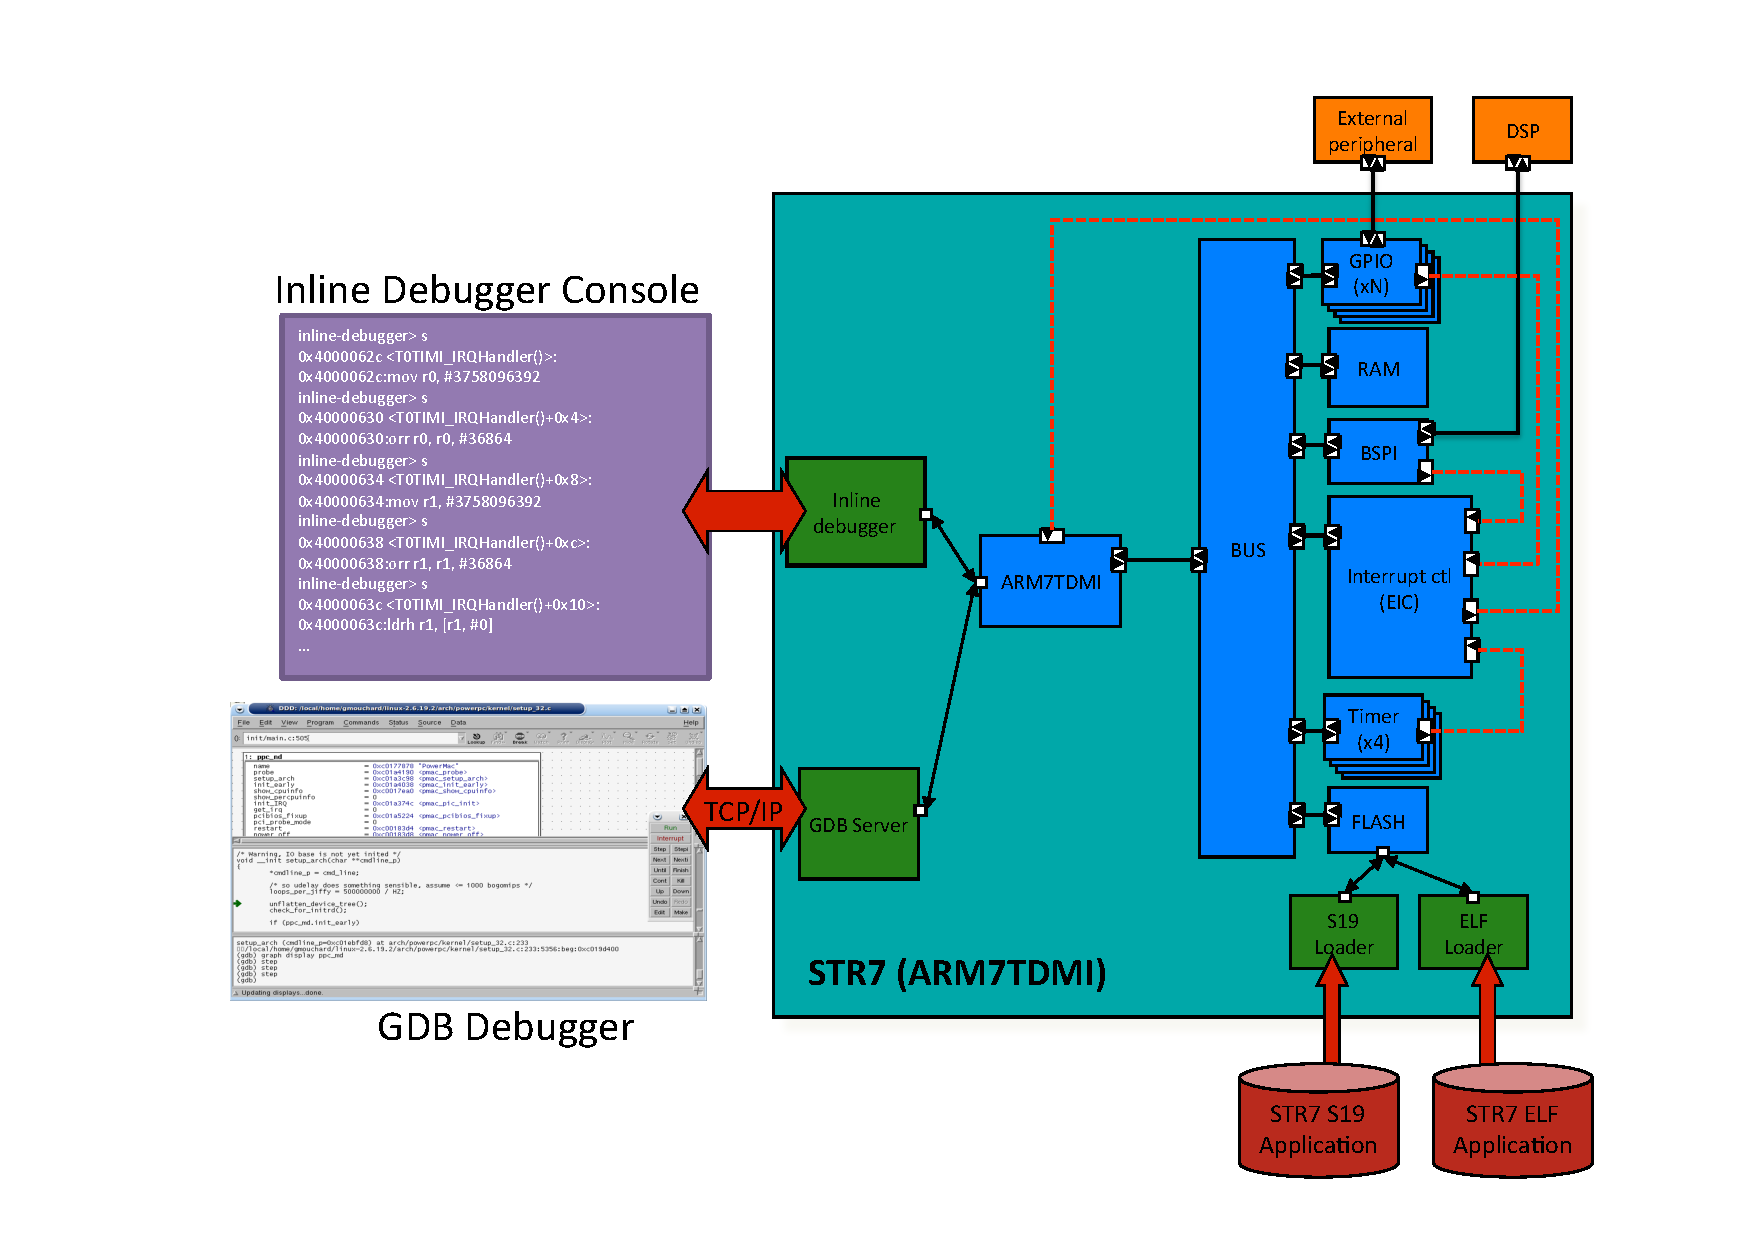
\includegraphics[width=\textwidth]{str7_validation/figures/str7_architecture.pdf}
	\end{center}
	\caption{STR7 schematic architecture.}
	\label{fig:str7_validation_str7_architecture}
\end{figure}

The ARM7TDMI architecture is based on \textit{Reduced Instruction Set Computer} (RISC) principles.
It uses a three-stage pipeline, so instructions are executed in three stages:
\begin{itemize}
	\item Fetch: instruction fetched from memory.
	\item Decode: decoding of registers used in instruction.
	\item Execute: register(s) read from register bank, shift and/or ALU operation, write register(s) back to register bank.
\end{itemize}
A total of 32 registers are available.
However, the processor has seven modes of execution, and while executing in a given mode the processor has only access to a subset (concretely sixteen registers) of them.
Additionally, the ARM7TDMI can execute two different instruction sets (ISAs):
\begin{itemize}
	\item Standard ARM ISA: it is composed of 32 bits RISC instructions. This is the main ISA of the ARM processors series.
	\item Thumb ISA: it is composed of 16 bits RISC instructions. This ISA is used to reduce code footprint, however the number of instructions proposed by this ISA is reduced, so not all kind of operations can done using this ISA.
\end{itemize}
The two ISAs are fully supported by the simulator.

The ARM7TDMI microprocessor is the base of the STR7 family.
The STR7 family extends it with the following peripherals (from the STR71X series):
\begin{itemize}
	\item Memories: Flash and RAM memories, and external memories are supported by the microcontroller.
	\item Nested interrupt controller with support of:
	\begin{itemize}
		\item fast interrupt handling with multiple vectors, 
		\item 32 vectors with 16 IRQ priority levels,
		\item and 2 maskable FIQ sources
	\end{itemize}
	\item Up to 48 I/O ports.
	\item 5 timers, including:
	\begin{itemize}
		\item a 16-bit watchdog
		\item 3 16-bit timers with 2 input captures, 2 output compares, PWM and pulse counter
		\item a 16-bit timer for timebase functions
	\end{itemize}
	\item 10 communication interfaces, including support for BSPI, CAN, and USB among others.
\end{itemize}

Not the complete STR7 system has been implemented under UNISIM, but a subset that includes:
\begin{itemize}
	\item memories,
	\item interrupt controller,
	\item basic GPIO functionality,
	\item timers (with the exception of the 16-bit watchdog),
	\item the BSPI communication interface,
	\item other components where replaced by stubs (ADC, I2C, APB, and PRCCU among others), because they were not used with the applications under test.
\end{itemize}
For the development of the STR7 simulator the following documents were used:
\begin{itemize}
	\item ARM Architecture Reference Manual
	\item ARM7TDMI (Rev 4) Technical Reference Manual
	\item STR71xF microcontroller family Reference Manual (UM0084)
\end{itemize}
Please refer to them if you are looking for more details on the ARM7TDMI processor and the STR7 microcontroller.

Figure~\ref{fig:str7_validation_str7_architecture} shows the schematic architecture of the simulator used for the validation of the STR7 microcontroller.
The simulator itself consist on the following components (the blue boxes on Figure~\ref{fig:str7_validation_str7_architecture}):
\begin{itemize}
	\item \textbf{ARM7TDMI:} this component models the ARM7TDMI processor.
	\item \textbf{System Bus:} this component allows the connection of the ARM7TDMI processor to the main memory.
	\item \textbf{RAM:} this component is the memory of the system. The processor uses it to store temporary information. It can be parametrized as a RAM or SRAM.
	\item \textbf{FLASH:} a flash type memory used by the microcontroller as boot. It is only as a read-only memory in the system under test.
	\item \textbf{GPIOs:} this component is used to perform communication with peripherals external to the microcontroller using the GPIO protocol.
	\item \textbf{BSPI:} this component is used to perform communication with peripherals external to the microcontroller using the SPI protocol.
	\item \textbf{Interrupt Controller:} this component synthesizes and prepares the different system interruptions before handling from the ARM7TDMI processor.
	\item \textbf{Timers:} a series of timers to perform time handling operations.
\end{itemize}

The simulator can be easily extended to use external modules thanks to the GPIO and the BSPI interfaces provided.
Additionally, the simulator provides two services (green boxes on Figure~\ref{fig:str7_validation_str7_architecture}):
\begin{itemize}
	\item \textbf{S19 Loader:} thanks to this service S19 STR7 binaries can be loaded into the FLASH/RAM component.
	\item \textbf{ELF Loader:} thanks to this service ELF STR7 binaries can be loaded into the FLASH/RAM component. The advantage of the ELF loader is that ELF binaries can contain debugging information (like symbols), unlike S19 binaries. This can be helpful when using the debugging tools.
	\item \textbf{GDB Server:} this service enables extended debugging with the help of an external client debugger, as for example: gdb, ddd, eclipse debugger, and others.
	\item \textbf{Inline Debugger:} this service incorporates an extended inline debugger tool to the simulator without the need of a client debugger.
\end{itemize}




\section{Tools}
\label{sec:tools}

For the validation of the STR7 simulator the following tools were used during the evaluation of the ARM7TDMI processor used on the STR7 microcontroller:
\begin{itemize}
	\item Random test generator: tool created at CEA to create random tests from an input template. It is briefly described in Section~\ref{sec:random_tests}.
	\item GNU compilations tools for ARM:
	\begin{itemize}
		\item GCC version 3.4.5 (C compiler)
		\item AS version 2.15 (Assembler compiler)
		\item LD version 2.15 (Linker)
	\end{itemize}
	\item GNU debugger for ARM: gdb version 6.1.1
	\item Linksys NSLU2 containing an ARM9 microprocessor. This is the target platform to validate the simulator against.
\end{itemize}

For the evaluation of the complete microcontroller the following tools were used:
\begin{itemize}
	\item STR7 evaluation board
	\item Schneider Electric software for the STR7 microcontroller generated using both the ARM RealView software and Code Composer
\end{itemize}


\section{User Level ISA Validation}
\label{sec:user_level}

When performing the validation of the ISA at the \emph{user level} we are only interested in the instructions that the processor can execute when running at the \emph{user mode}.
The \emph{user mode} is usually the most used mode on a processor (whenever the processor has multiple execution modes, which the ARM7TDMI has).
It is used to run the non-system dependent part of the applications.
Whenever an application needs to access the system (write on the screen, read the input from the keyboard, etc), it executes an special instruction (usually we call it \textit{system call}) which switches the processor to \emph{system mode} to perform the required operation.

The interest on performing a validation of \emph{user level} instructions resides on the difficulty to perform complete tests when using the \emph{system level} instructions (as we will see on Section~\ref{sec:system_level}).

\begin{figure}[!h]
	\begin{center}
		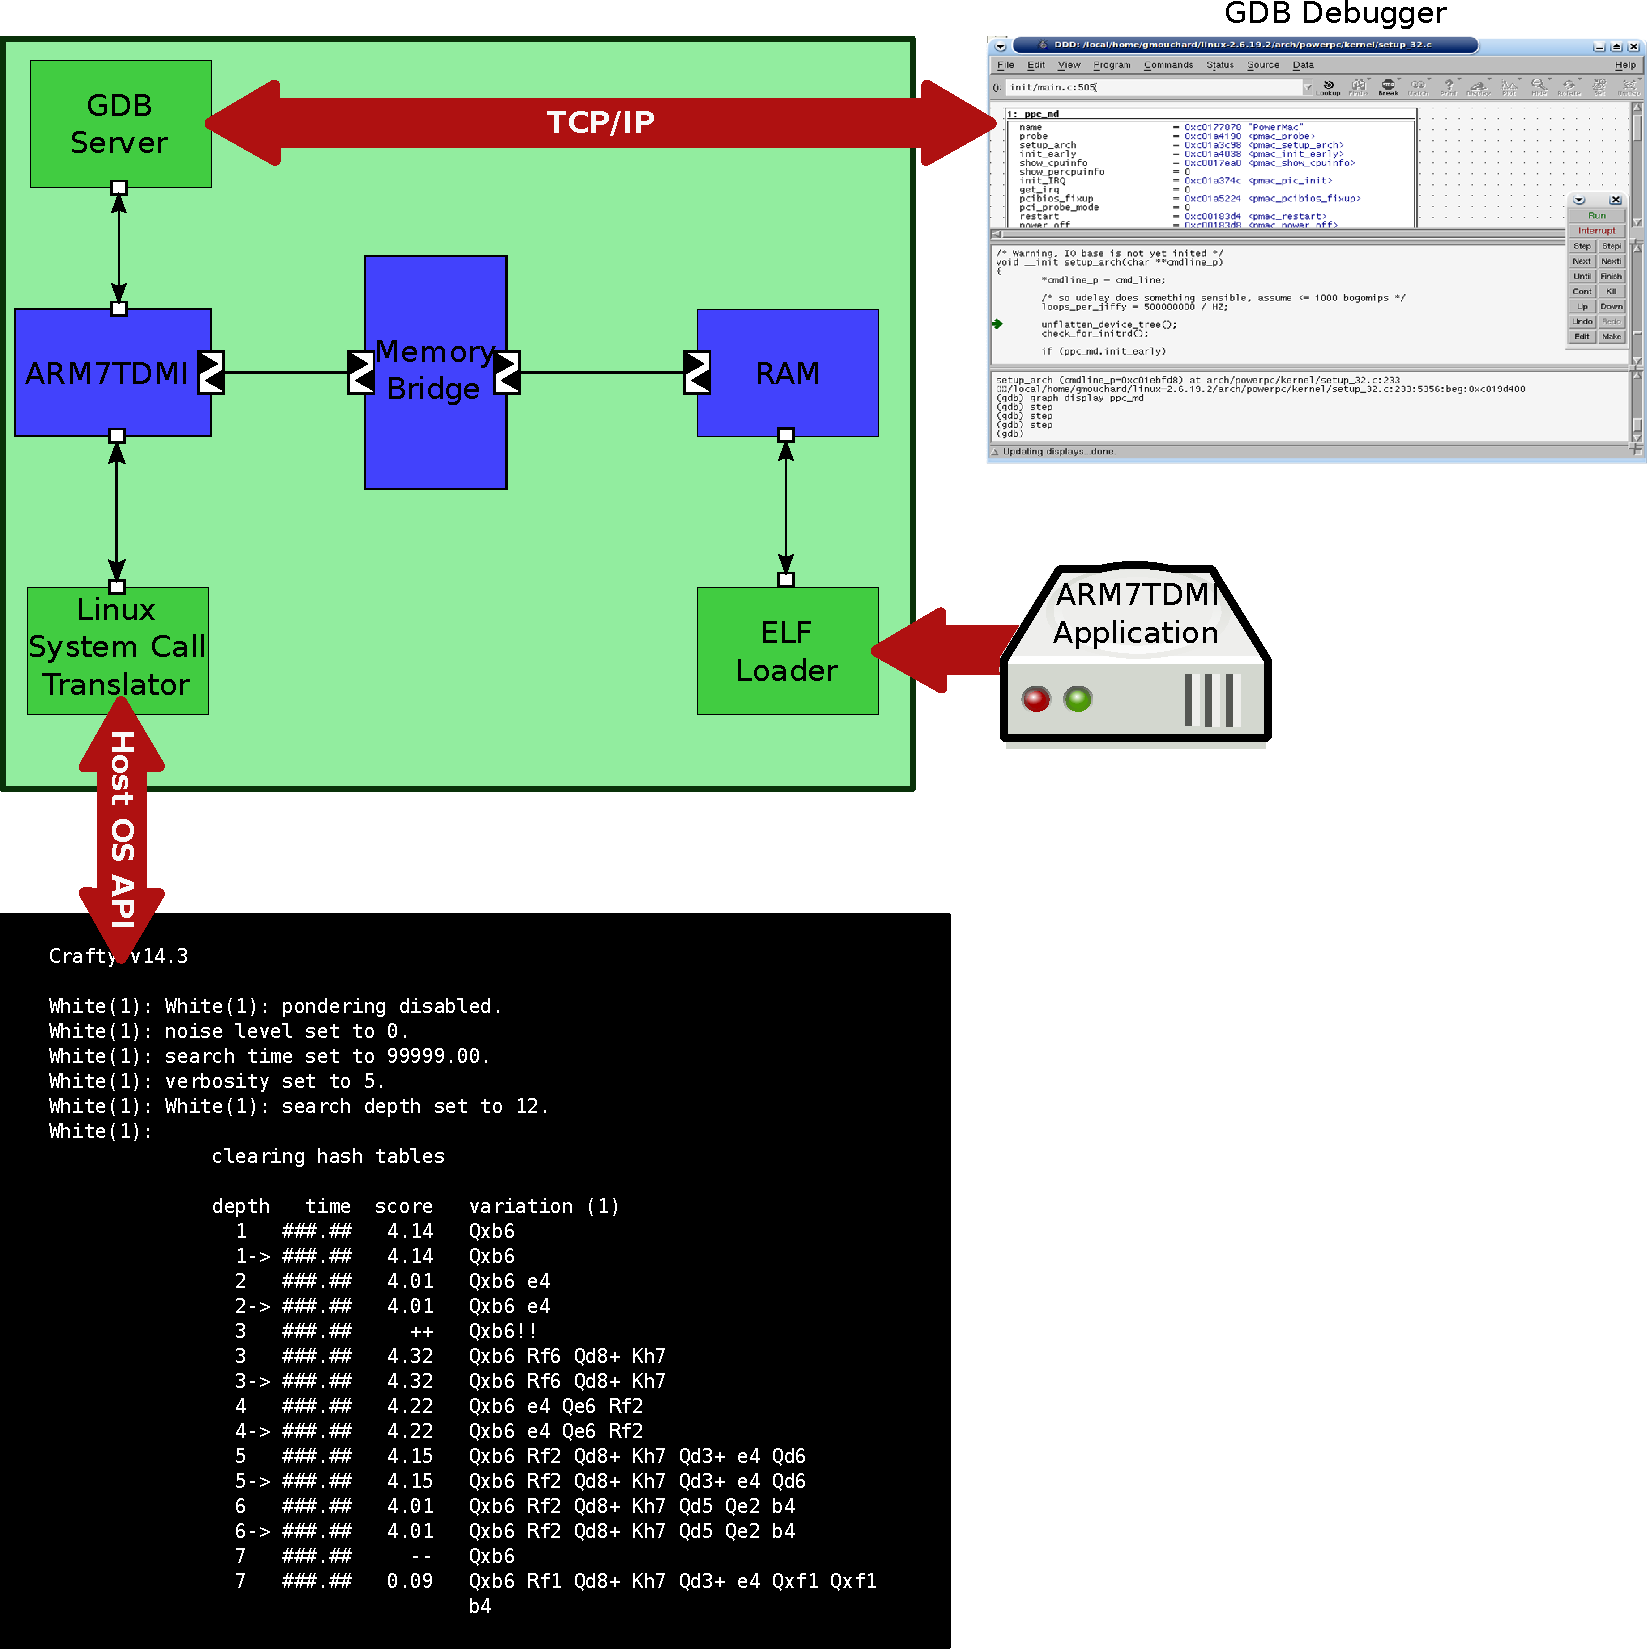
\includegraphics[width=\textwidth]{figures/ARM7TDMI_user_level.pdf}
	\end{center}
	\caption{ARM7TDMI schematic architecture to run applications at user level.}
	\label{fig:arm7tdmi_user_level}
\end{figure}

In order to validate only the \emph{user level} ISA, the simulator is run with a special configuration, see Figure~\ref{fig:arm7tdmi_user_level}.
To the \emph{ELF Loader} and the \emph{GDB Server} services a third service has been added: the \emph{Linux System Call Translator}.
This service takes control of the simulation when a system call is executed, providing the program being executed by the simulator a translation of the system calls, without having to execute any system level instruction.
More concreatelly, the \emph{Linux System Call Translator} provides a traduction to Linux programs, which means that programs running under this configuration need to be compiled for ARM Linux.

\begin{figure}[!h]
	\begin{center}
		\includegraphics[width=\textwidth]{figures/random_tests_methodology.pdf}
	\end{center}
	\caption{Random tests methodology.}
	\label{fig:random_tests_methodology}
\end{figure}

Figure~\ref{fig:random_tests_methodology} shows the steps taken to perform the validation of the user level ISA.
Once the simulator is written an application is run into booth the simulator and the target platform.
The output results of the simulator and the target platform are then compared.
If results match then it means that the simulator is correctly implemented.
If the results do not match we debug the simulator to fix it using the results differences, and the previous steps are repeated until the results match.

The following two subsections presents different validation tests performed under this configuration.
As target platform we used an ARM9 platform.
While it is not an ARM7TDMI platform, the ARM9 shares the same instructions at the user level, making it a valid target platform for the ARM7TDMI simulator at the user level.

\subsection{Random Tests}
\label{sec:str7_validation_random_tests}

The validation of all the instructions is an impossible task as it would mean to check all the instructions with all the possible inputs.
So in order to create an extensive and systematic validation of all the instructions we have created a small tool to generate random tests.
The tool takes as input a template describing the instruction to test, but not defining the instruction inputs.
The tool then creates multiple tests of the instruction defining random inputs.
The outputs of the tests are printed on the screen, so we can compare the outputs of the simulator against those of the target platform.

\begin{figure}[!h]
	\input{str7_validation/adc_imm}
	\caption{\texttt{adc} with immediate input template.}
	\label{fig:str7_validation_adc_imm_template}
\end{figure}

Figure~\ref{fig:str7_validation_adc_imm_template} shows an example of template for the \texttt{adc} instruction using an immediate as input.
Line \texttt{1} sets to 0 the \texttt{r9} register which will be used later for storing the result of the \texttt{adc} instruction.
Lines \texttt{2}, \texttt{3} and \texttt{4} set randomly the status bits of the \texttt{cpsr} register which may influence the computation of the \texttt{adc} instruction.
Line \texttt{5} is the actual test of the \texttt{adc} instruction. 
The \texttt{\%(,eq,ne,...)} string appends nothing or one of the guarding pnemonics to the \texttt{adc} instruction, which one is selected randomly by the random tests generator.
Similarly the \texttt{\%(,s)} string appends nothing or the ``\texttt{s}'' string to the \texttt{adc} instruction.
The ``\texttt{s}'' flag indicates that the \texttt{cpsr} register should be updated if present, or leaved untouched otherwise.
The result of the \texttt{adc} instruction is stored in the \texttt{r9} register.
The \texttt{adc} uses two different inputs: a register and an immediate.
The register input is generated randomly by the test generator with the ``\texttt{\%r}'' string, choosing randomly one of the available registers and setting it to a random generated value.
The immediate input is generated randomly with the ``\texttt{\%s8,4,2}'' string\footnote{We are not going to get into details on how the immediate value is defined, just mention that it generates an integer that can be accepted by the ARM7 compiler.}.
Finally, lines \texttt{6}, \texttt{7} and \texttt{8} store the maybe modified \texttt{cpsr} status flags into a register chosen by the test generator (indicated with the ``\texttt{\%R}'').
Similarly, in line \texttt{9}, the register \texttt{r9} is copied into a register chosen by the test generator.
The registers marked with the ``\texttt{\%R}'' are then printed into the terminal, so we can compare the outputs from the simulation and the execution on ARM9 platform.
For each instruction test we check that the output register and the \texttt{cpsr} flags are correctly set.

\subsubsection{Results}

Test templates as the one presented in Figure~\ref{fig:str7_validation_adc_imm_template} have been developed for all the versions of the \texttt{adc} instruction (i.e., with two input registers, with a shifted immediate as input, and with a shifted register as input), and for all of the versions of most of the \textit{user level} instructions of the ARM7TDMI.
A total of 100,000 tests were generated from each template (making an average of 400,000 tests for instruction), and all the tests were succesfully passed. The following is a list of the validated instructions:
\begin{enumerate}
	\item adc
	\item add
	\item and
	\item bic
	\item cmn
	\item cmp
	\item eor
	\item mla
	\item mov
	\item mul
	\item mvn
	\item orr
	\item rsb
	\item rsc
	\item sbc
	\item smlal
	\item smull
	\item sub
	\item teq
	\item tst
	\item umlal
	\item umull
\end{enumerate}

This list includes all the \textit{user level} instructions of the ARM7TDMI processor, with the exception of memory instructions, branch instructions, and the system call instruction.
To validate those instructions (and complete the validation of the \textit{user level} instructions tested by the random tests), we performed tests over full applications presented in the following section.


\subsection{Benchmark Suite}
\label{sec:benchmark_suite}

While the validation performed in the previous section ensures the correct individual behavior of the tested instructions, it does not test the interaction between them, and some instructions are still missing, like all the load/store instructions, branch instructions, and the system call instruction.
To test the missing instructions and their interactions different real world applications are better suited.

The applications used for this validation are the SPEC2000 CINT.
The following is a list of the applications used with a small description extracted from the SPEC2000 documentation:
\begin{itemize}
	\item \textbf{gzip:} gzip (GNU zip) is a popular data compression program written by Jean-Loup Gailly $<$gzip@gnu.org$>$ for the GNU project. gzip uses Lempel-Ziv coding (LZ77) as its compression algorithm.
	\item \textbf{vpr:} VPR is a placement and routing program; it automatically implements a technology-mapped circuit (i.e. a netlist, or hypergraph, composed of FPGA logic blocks and I/O pads and their required connections) in a Field-Programmable Gate Array (FPGA) chip.  VPR is an example of an integrated circuit computer-aided design program, and algorithmically it belongs to the combinatorial optimization class of programs.
	\item \textbf{gcc:} this application is based on gcc Version 2.7.2.2. It generates code for a Motorola 88100 processor. The benchmark runs as a compiler with many of its optimization flags enabled.
	\item \textbf{mcf:} a benchmark derived from a program used for single-depot vehicle scheduling in public mass transportation. The program is written in C, the benchmark version uses almost exclusively integer arithmetic.
	\item \textbf{crafty:} Crafty is a high-performance Computer Chess program that is designed around a 64bit word. It runs on 32 bit machines using the ``long long'' (or similar, as \_int64 in Microsoft C) data type.  It is primarily an integer code, with a significant number of logical operations such as and, or, exclusive or and shift.  It can be configured to run a reproducible set of searches to compare the integer/branch prediction/pipe-lining facilities of a processor.
	\item \textbf{parser:} parser does the grungy job of chopping the user's input sentence into words, processing the special commands, and calling all the functions necessary to parse the input sentence.
	\item \textbf{eon:} Eon is a probabilistic ray tracer based on Kajiya's 1986 ACM SIGGRAPH conference paper. It sends a number of 3D lines (rays) into a 3D polygonal model. Intersections between the lines and the polygons are computed, and new lines are generated to compute light incident at these intersection points. The final result of the computation is an image as seen by camera. The computational demands of the program are much like a traditional deterministic ray tracer as described in basic computer graphics texts, but it has less memory coherence because many of the random rays generated in the same part of the code traverse very different parts of 3D space.
	\item \textbf{perlbmk:} perlbmk is a cut-down version of Perl v5.005\_03, the popular scripting language. SPEC's version of Perl has had most of OS-specific features removed.
	\item \textbf{gap:} gap implements a language and library designed mostly for computing in groups (GAP is an acronym for Groups, Algorithms and Programming).
	\item \textbf{vortex:} VORTEx is a single-user object-oriented database transaction benchmark  which which exercises a system kernel coded in integer C.
	\item \textbf{bzip2:} bzip2 is based on Julian Seward's bzip2 version 0.1. The only difference between bzip2 0.1 and bzip2 is that SPEC's version of bzip2 performs no file I/O other than reading the input. All compression and decompression happens entirely in memory. This is to help isolate the work done to only the CPU and memory subsystem.
	\item \textbf{twolf:} The TimberWolfSC placement and global routing package is used in the process of creating the lithography artwork needed for the production of microchips. Specifically, it determines the placement and global connections for groups of transistors (known as standard cells) which constitute the microchip. The placement problem is a permutation. The TimberWolfSC program (twolf) uses simulated annealing as a heuristic to find very good solutions for the row-based standard cell design style.  In this design style, transistors are grouped together to form standard cells.
\end{itemize}

All these applications were developed in order to stress the cpu and the memory system, which covers the memory and branch instructions validation missing in the random tests presented in Section~\ref{sec:random_tests}. 
Additionally, while not in an intensive manner, those applications test the functionality of the system call instruction.

\subsubsection{Results}

All those applications have been successfully run in the ARM7TDMI simulator, and their outputs match those of to the target plaform.
Three different input sets (provided with the SPEC2000) have been used for each of the application:
\begin{itemize}
	\item \textbf{train:} small input set that has been mainly used during the development of the simulator.
	\item \textbf{test:} medium size input set.
	\item \textbf{ref:} large size input set, recommended by the SPEC2000 manual to fully stress the CPU and the memory system.
\end{itemize}

All the SPEC2000 applications were used during the development of the simulator, and no other tests were performed until all of them were successfully simulated.
After that the random tests (see Section~\ref{sec:random_tests}) were performed founding only one error (with the \texttt{mrc} instruction).
Finally, the system test presented in the following Section were performed to validate the system level behavior of the ARM7TDMI simulator.




\section{System Level Validation}
\label{sec:system_level}

The tests presented in Section~\ref{sec:user_level} validated the user level ISA subset of the complete ARM7TDMI ISA.
Validation of the system level ISA is a more complicated.
Firstly, systematic tests as the random tests introduced in Section~\ref{sec:random_tests} are not feasible, due to the system dependencies of those instructions.
Secondly, there are not benchmarks as those presented in Section~\ref{sec:benchmark_suite} to validate the ARM7TDMI alone.
System benchmarks exist, but they require more components than those developed for the architecture targeted in this document (see Figure~\ref{fig:arm7tdmi_architecture}).

For those reasons we have developed a small kernel to test the following features of the system:
\begin{itemize}
	\item system bootup
	\item exception mechanism
	\item user/system mode switching
	\item ARM ISA to Thumb ISA switching
\end{itemize}

\subsection{Results}
To validate the behavior of the ARM7TDMI simulator at system level we do not have any tool to do it automatically (we can not compare two outputs like presented in Section~\ref{sec:user_level}).
We performed all the validation manually, heavily using the debugging service provided with UNISIM and comparing the behavior of the simulator to the behavior described in the ARM manual.
All the tests were succesfully validated.


\section{Microcontroller validation}
\label{sec:str7_validation_microcontroller_validation}

The previous sections focused on the validation of the ARM7TDMI processor simulator at user and system level.
In this section, the target of the validation is the complete microcontroller under study\footnote{We would like to thank Schneider Electric, and specially Khaled Rahmouny for his collaboration on the validation of the UNISIM STR7 microcontroller simulator. Without their collaboration, the validation of the simulator on an industrial environment could not have been possible. For confidentiality issues the applications used during the validation and modules added on the simulator are not discussed in this document.} (see Figure~\ref{fig:str7_validation_str7_architecture}).
In order to validate the microcontroller a full application that boots the device and uses the different peripherals was necessary, and preferably a real world application.
For that purpose Schneider Electric has provided the software necessary to run the microcontroller and extended the simulator desing with an external DSP and a graphical interface of the Schneider Electric product embedding the STR7 microcontroller.

\begin{figure}[!h]
	\begin{center}
		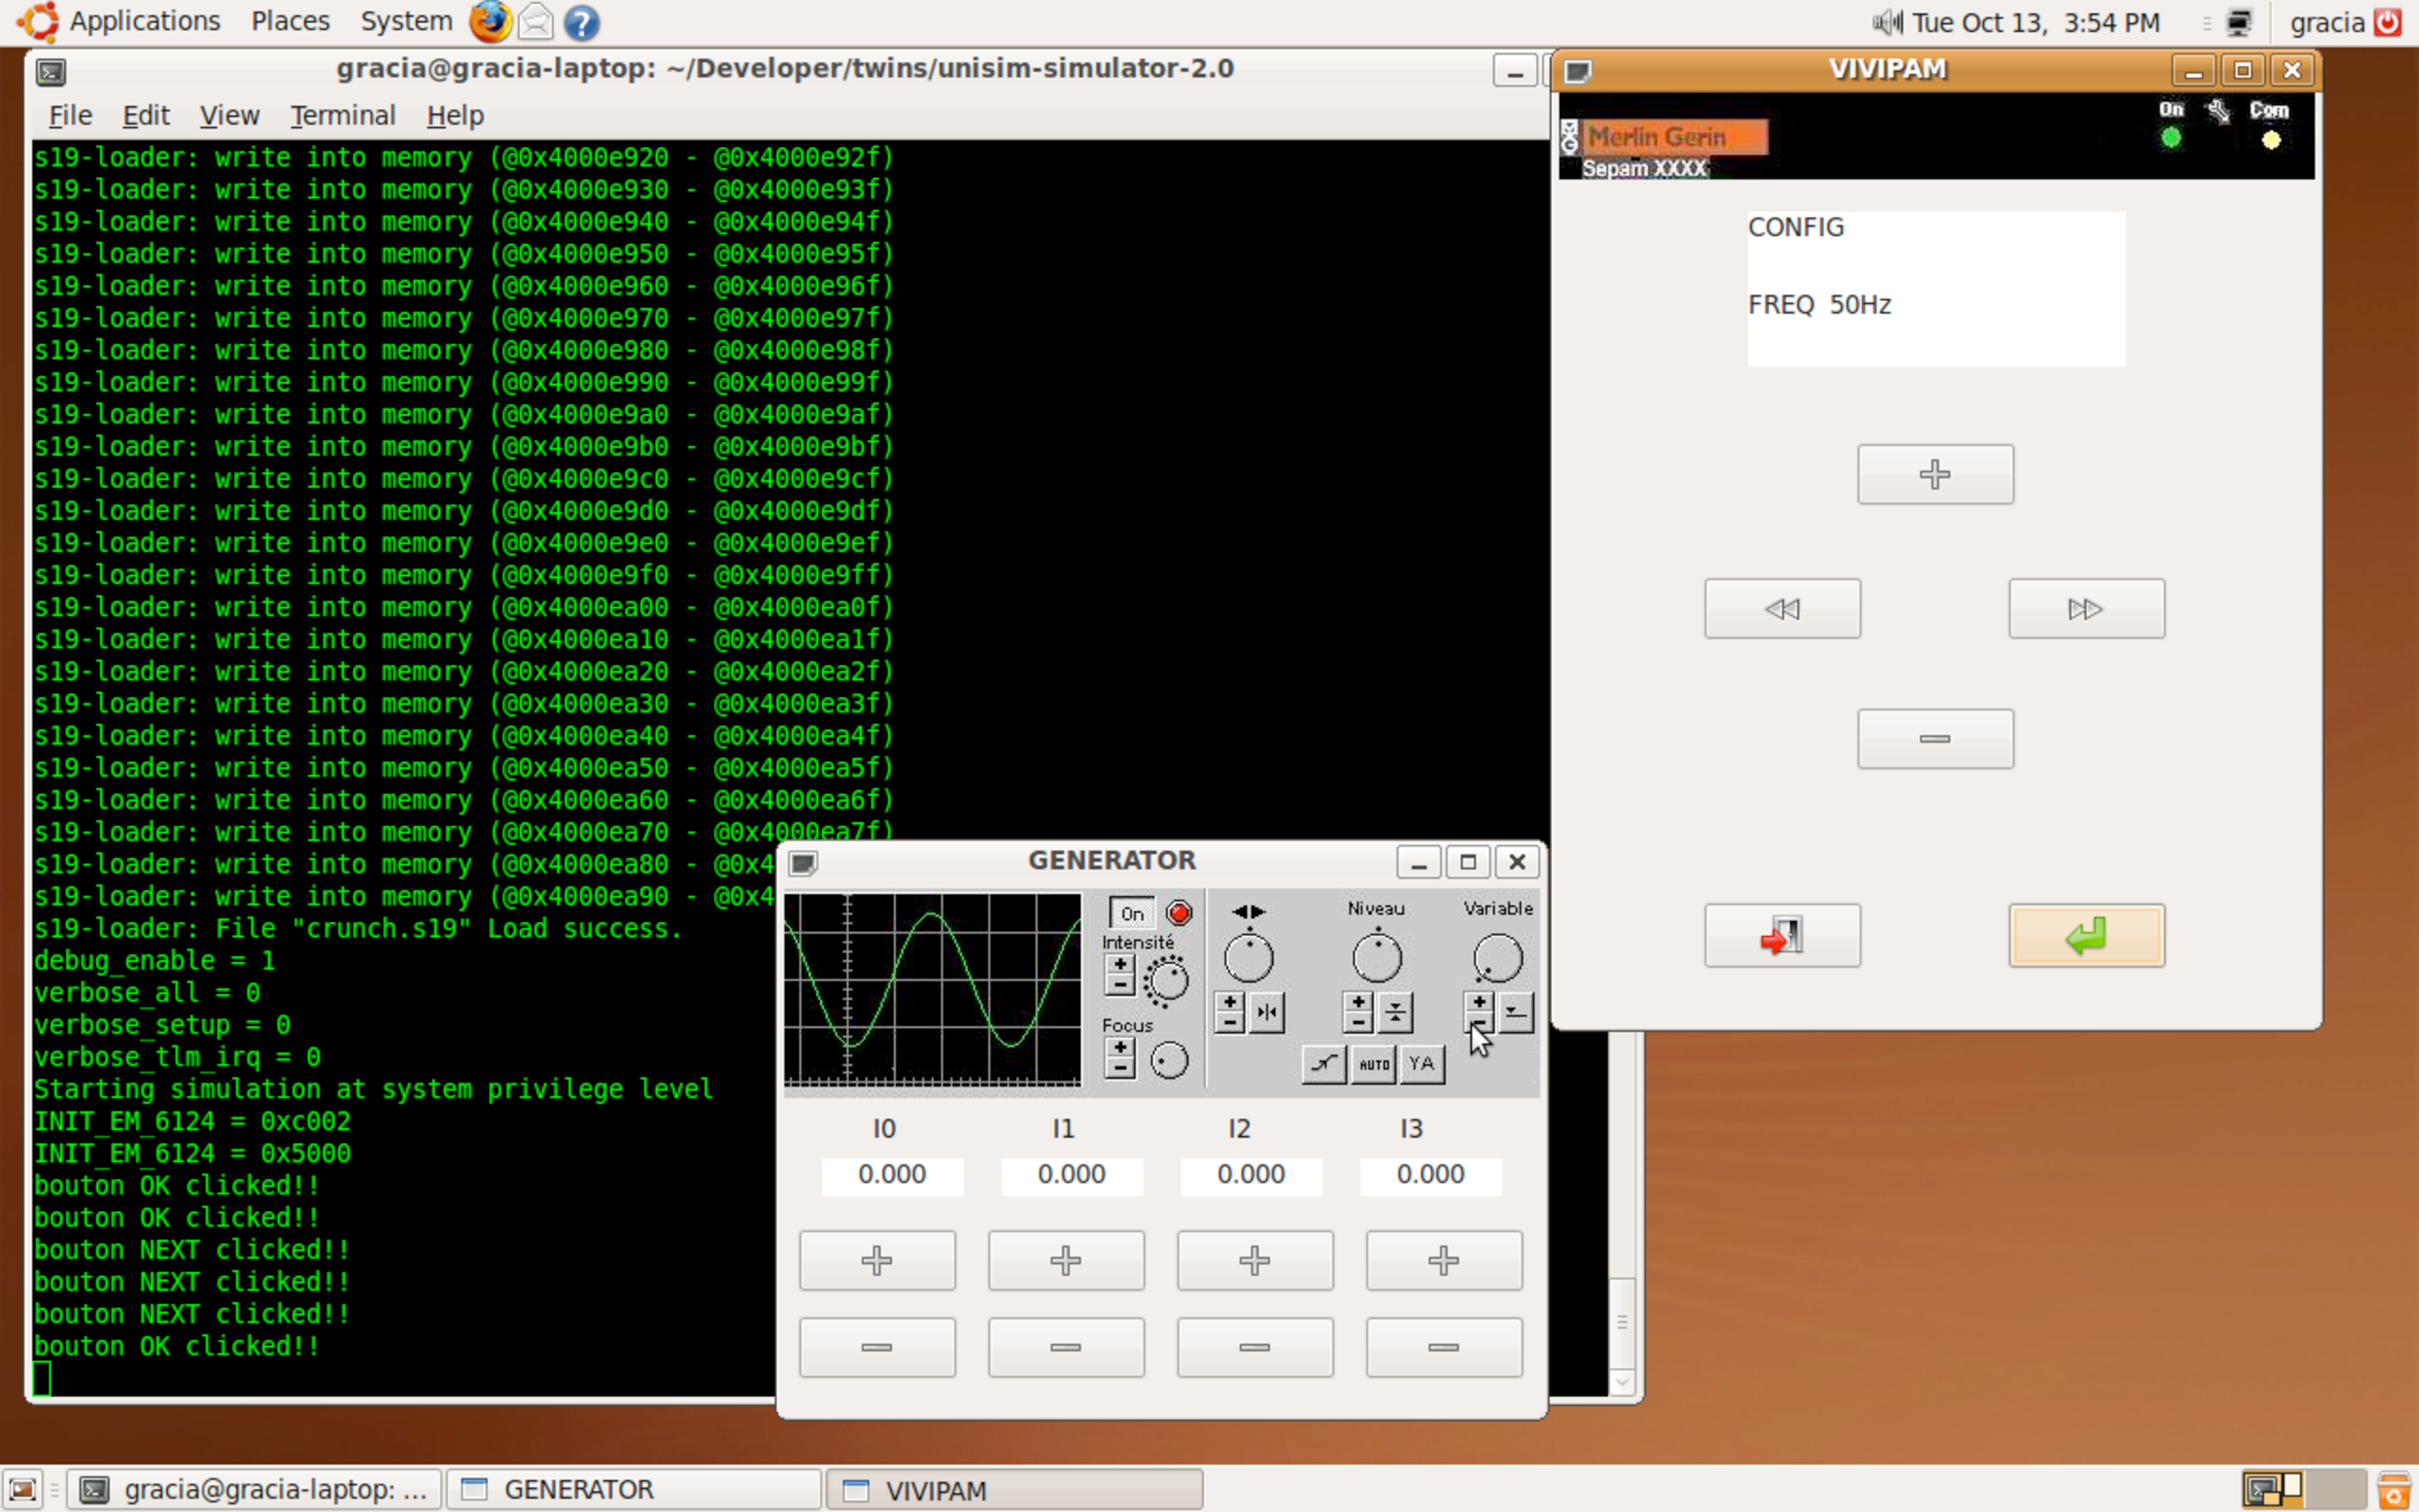
\includegraphics[width=\textwidth]{str7_validation/figures/industrial.pdf}
	\end{center}
	\caption{Industrial application running on top of the STR7 simulator.}
	\label{fig:str7_validation_industrial_application}
\end{figure}

The validation of the microcontroller has been done progressively and all the capabilities of the simulator were tested.
The steps followed during the validation were:
\begin{enumerate}
	\item ELF and S19 loaders test.
	\item Microprocessor boot process validation.
	\item Validation of bus communications, mainly with the RAM and the FLASH memories.
	\item Procesor validation using a regression test software used by Schneider Electric.
	\item Validation of the interruption handling, this includes the both the processor and the interrupt controller.
	\item Timers capabilities validation.
	\item Validation of the BSPI communication peripheral. For this test the BSPI peripheral was connected to the external DSP developed by Schneider Electric.
	\item Validation of the GPIO peripherals.
	\item Validation of the complete system using a industrial application.
\end{enumerate}
For each of the validation steps a STR7 software provided by Schneider Electric was used, which was augmented as each step validation was successfully passed.
Figure~\ref{fig:str7_validation_industrial_application} shows the final program running on top of the simulator.

The functional behavior of the simulator of the microcontroller simulator was validated against a real system using the same STR7 microcontroller.
Additionally timing tests were run to check the time precision of the simulator.

\subsection{Results}

The functional behavior of the different components of the simulator and of the simulator as a whole has been validated, thanks to the use of the industrial application.

The timing behavior currently differs with the real platform. 
Our tests showed that the simulated software is slightly slower than on the real platform.
However, the slightly different timings do not impact on the development of industrial applications over the simulator.



\section{Conclusion}
\label{sec:conclusion}

This document has presented the different tests that have been performed in order to validate the ARM7TDMI simulator.
With the SPEC2000 application suit the simulator have been validated to be used with real world applications.
Thanks to the random tests technique developped at CEA an extensive validation of all the ARM7TDMI user level instructions have been done.
Finally, with the development of a small kernel the simulator has been validated for the execution of system level applications, like operating systems, drivers, and embedded applications.

As for any software application, the validation does not ensure that the simulator is bug free.
However, the validation performed ensures that the simulator functionality matches the ARM7TDMI functionality, and that any application can be run on it with confidence.
Additionally, the ARM7TDMI simulator provided in UNISIM (http:$\backslash\backslash$www.unisim.org) is open source, which means that users can fixe it if necessary and that corrections to the simulator can be easily shared.



\end{document}

